\chapter[Software]{Software}

    \section[WebService]{WebService}

        A demanda do problema exige que diferentes hardwares se integrem com uma
        mesma base de dados. Fundamentalmente, o Smartphone do usuário realiza a compra, e
        o token deve reconhecer o QrCode para que o usuário consuma o chopp.
        
        Para solucionar essa demanda foi proposto uma arquitetura orientada a serviços
        (SOA), tal que uma webservice REST seja responsável pela persistência e autenticação de todos os
        dados relevantes do sistema, incluindo a autenticação de pagamentos.

        A tecnologia escolhida para implementação desse sistema foi o framework o 
        Ruby On Rails\footnote{\url{http://rubyonrails.org/}}, pela facilidade no desenvolvimento, 
        ampla comunidade e experiência da equipe. Sendo o Ruby na versão 2.3.0 e o Rails na versão 5.0.5.

        Para autenticação de pagamentos foi utilizada a API do PagSeguro\footnote{\url{https://github.com/pagseguro/ruby}},
        que recebe as requisições do WebService com os dados do comprador e registra a transação caso os dados estejam corretos,
        ou retorna erros, caso contrário. Quando o pagamento dessa transação muda de status, ou seja, é aprovado, o PagSeguro
        manda uma notificação de volta para o WebService de modo que assim possa ser gerado o QRCode.

        A persistência dos dados ocorre seguindo o modelo abaixo:

        \begin{figure}[H]
            \centering
            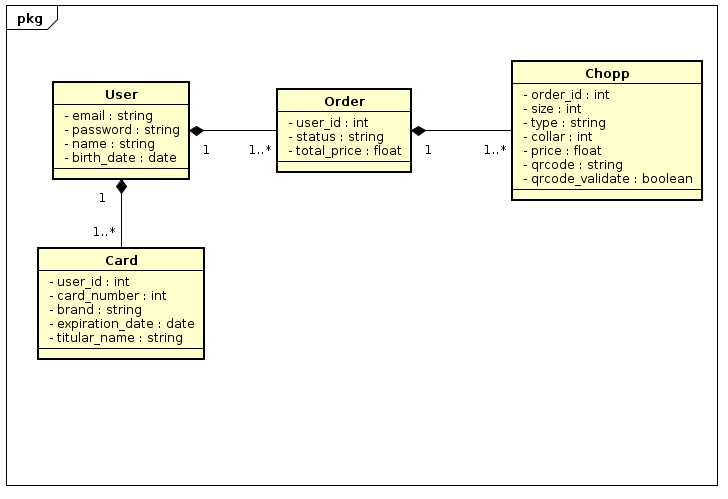
\includegraphics[scale= 0.4]{figuras/Diagrama-de-classes.png}
            \caption{Modelagem. Fonte: Própria.}
            \label{modelagem}
        \end{figure}

        Para hospedagem do WebService foi usado o Heroku\footnote{\url{https://www.heroku.com/}}.
        As vantagens em utilizar essa plataforma estão no custo, 
        por ser uma ferramenta grátis e na facilidade de fazer o deploy.

    \section[Sistema Administrativo]{Sistema Administrativo}

        O Sistema administrativo está incorporado ao aplicativo do Sistema de Compras, porém apenas usuários
        administradores possuem acesso. Ao utilizar o aplicativo, o usuário visualiza
        as seguintes informações referentes ao estado da máquina: a quantidade de chopp que a
        máquina possui, a temperatura de resfriamento e o status da conexão da máquina com a internet.

        Esses valores são recuperados através de requisições GET ao WebService que guarda essas informações recebendo
        requisições POST a cada 60 seg da aplicação que lê os dados dos sensores. 
    
    \section[Sistema de Validação de Compra]{Sistema de Validação de Compra}
        
        O sistema de validação se trata do módulo responsável pela validação dos dados da compra,
        e dar o inicio no processo de serventia de chopp conforme as característias são pré-definidas.
        Esse subsistema tinha como resultados esperados uma aplicação que pudesse prover ao usuário
        a leitura do \textit{QRCode} gerado no momento da compra do chopp por meio de uma câmera 
        acoplada na máquina de onde o chopp é armazenado. No \textit{QRCode} estão contidas as informações
        referentes as preferências do consumidor no que tange sua bebida.
        
        Devido à necessidade de que o usuário tenha acesso a uma câmera para leitura do \textit{QRCode},
        foi escolhido o \textit{framework} Python Kivy\footnote{\url{https://kivy.org/}} por fornecer um ambiente
        \textit{touchscreen} com um baixo consumo de recursos, uma vez que essa aplicação estará 
        instanciada em uma Raspberry responsável por gerenciar outros módulos operacionais do projeto.

        Desta forma, foi então desenvolvida aplicação Autochopp-Machine \footnote{\url{https://github.com/autochopp/autochopp-machine}} que fornece de forma interativa 
        com a validação de \textit{QRCodes} e iniciação do processo de retirada do chopp. 

        Além do que foi citado, a aplicação também possui a responsabilidade de fazer requisições junto a API
        para que a mesma possa informar se o \textit{QRCode} lido é válido, significando que a compra foi 
        efetuada com sucesso, caso não śeja válido, é exibida uma mensagem de erro. A partir da combinação
        de preferências feitas no momento da compra, é gerado um identificador que é vinculado ao 
        \textit{QRCode}. Esse identificador é o responsável por passar as informações via socket para que
        os componentes eletrônicos vinculados a máquina sejam capazes de atuar na composição do chopp conforme
        suas especificações.

        \begin{figure}[H]
            \centering
            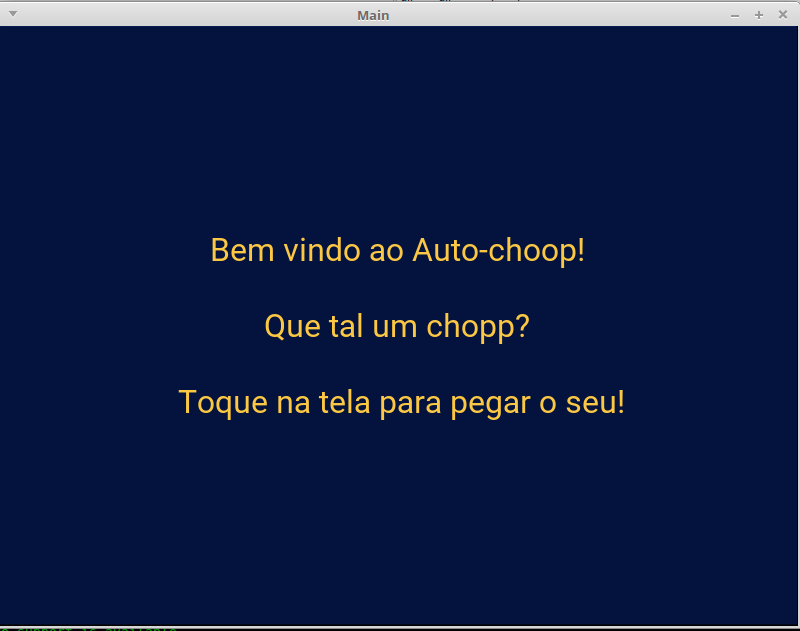
\includegraphics[scale= 0.4]{figuras/home-screen.png}
            \caption{Tela Inicial. Fonte: Própria.}
            \label{home-screen}
        \end{figure}

        \begin{figure}[H]
            \centering
            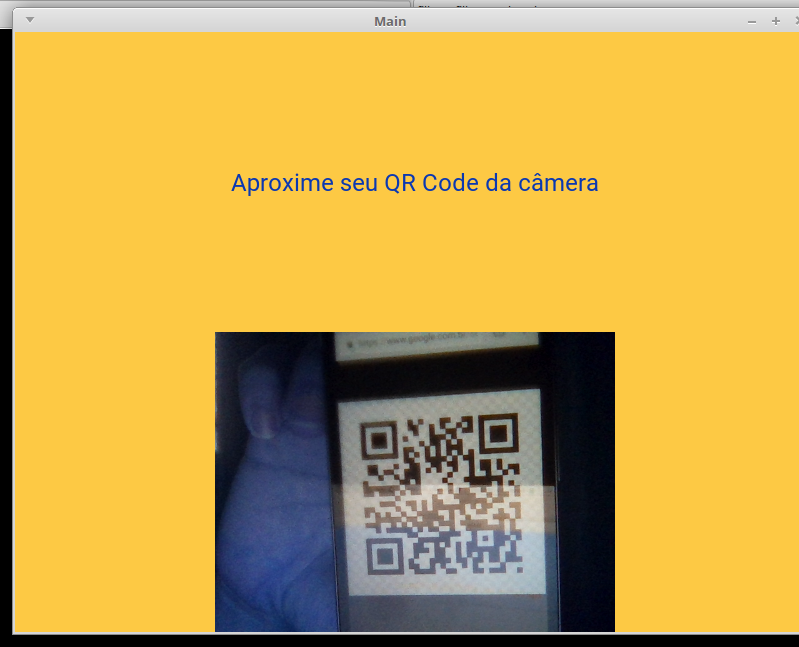
\includegraphics[scale= 0.4]{figuras/leitor-qrcode.png}
            \caption{Tela de Leitura de \textit{QRCode}. Fonte: Própria.}
            \label{leitor-qrcode}
        \end{figure}

        \begin{figure}[H]
            \centering
            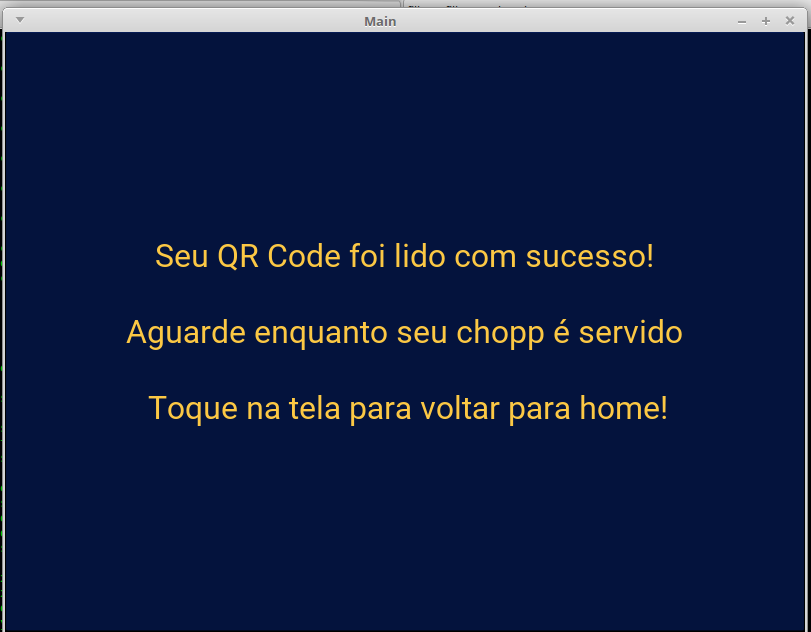
\includegraphics[scale= 0.4]{figuras/sucesso.png}
            \caption{Tela informando que o \textit{QRCode} foi lido com sucesso. Fonte: Própria.}
            \label{sucesso}
        \end{figure}

        \begin{figure}[H]
            \centering
            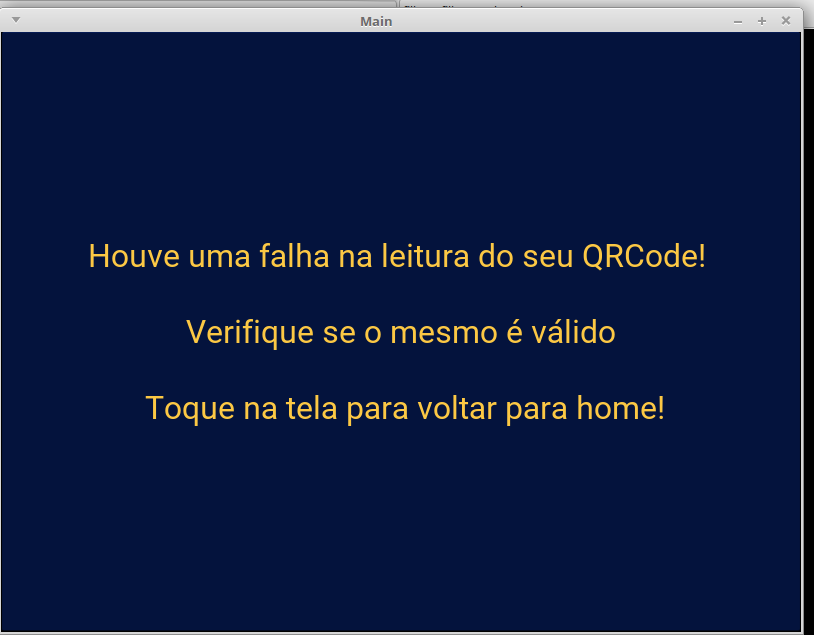
\includegraphics[scale= 0.4]{figuras/falha.png}
            \caption{Tela informando que o \textit{QRCode} não foi lido com sucesso. Fonte: Própria.}
            \label{falha}
        \end{figure}
    
        
\section[Aplicativo Mobile]{Aplicativo Mobile}

Para compra e gerenciamento dos cupons de \textit{chopp}, torna-se necessário um aplicativo \textit{mobile} de forma que seja facilitado a acessibilidade para os usuários.

\subsection{Requisitos do Projeto}

\subsubsection{Comprar Chopp}

\textbf{Dado} que o usuário esteja logado

\textbf{Quando} tenha iniciado a compra de um chopp

\textbf{Então} deve ser possível ver as preferências de chope(colarinho, quantidades discretas e pré-definidas)

\subsubsection{Cadastrar Usuário}

\textbf{Dado} que o usuário tente entrar no sistema 

\textbf{E} ainda não tenha se cadastrado

\textbf{Quando} tenha iniciado o aplicativo

\textbf{Então} terá disponível um formulário com email e senha para cadastro

\subsubsection{Confirmar Cadastro}

\textbf{Dada} que o usuário já tenha se cadastrado

\textbf{E} recebido um email com link de confirmação

\textbf{Quando} clicar no link

\textbf{Então} deverá ser levado a uma mensagem de confirmação

\textbf{E} deve ser possível se autenticar no sistema.

\subsubsection{Finalizar Compra}

\textbf{Dado} que o usuário já esteja cadastrado no sistema

\textbf{E} tenha clicado para comprar um chopp

\textbf{E} tenha acesso a internet

\textbf{Quando} finalizado a compra

\textbf{Então} deve ser possível inserir os dados do cartão de crédito

\textbf{E} ser notificado se a compra foi bem sucedida ou não

\textbf{E} em seus tickets devem estar disponíveis para uso na máquina

\subsubsection{Listar Cupons(QRCode)}

\textbf{Dado} que o usuário já tenha comprado tickets

\textbf{E} esteja autenticado no sistema

\textbf{Quando} clicar em uma opção meus tickets

\textbf{Então} deve ser possível  visualizar o QRCode que representa a unidade de chopp

\textbf{E} deverá ter disponível uma opção para usar o ticket

\textbf{E} caso já tenha sido usado o ticket, deverá sumir da lista de tickets do usuário

\subsubsection{Efetuar Compra Offline}

\textbf{Dada} a compra efetuada de um chopp

\textbf{E} um usuário offline

\textbf{Quando} o usuário clicar para usar o ticket

\textbf{Então} a máquina de chopp deve responder no sistema de interação com mensagem sucesso.

\subsubsection{Visualizar Cupon(QRCode)}

\textbf{Dado} que o usuário tenha comprado tickets

\textbf{Quando} entrar na tela de visualização de tickets

\textbf{Então} deve ser possível ver os tickets comprados segundo as preferências

\textbf{E} poder escolher qual queira consumir

\subsection{Projeto}

De acordo com os critérios observados do público alvo e do contexto considerado, pensou-se em um aplicativo mobile que se comunica com um Web Service para realizar as operações descritas na especificação acima.

\subsection{Casos de Teste}

Achar os casos de teste especificados no PC1...

\subsection{Solução Adotada}

Por fim, foi desenvolvido um aplicativo multiplataforma utilizando o \textit{framework Ionic 3}, baseado em \textit{Angular 4}. As imagens das telas do aplicativo estão na Figura \ref{telasapp1} e \ref{telasapp2}.

\begin{figure}[H]
\centering
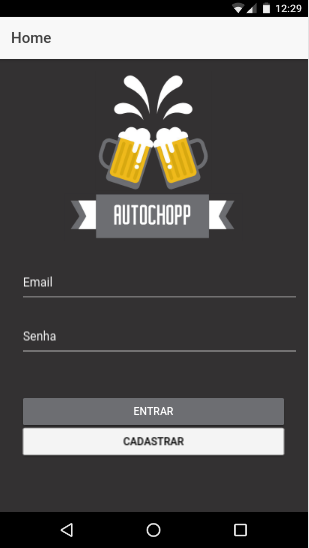
\includegraphics[scale= 0.4]{figuras/homepage.png}
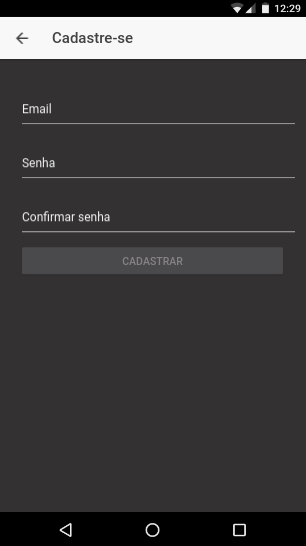
\includegraphics[scale= 0.4]{figuras/signup.png}   
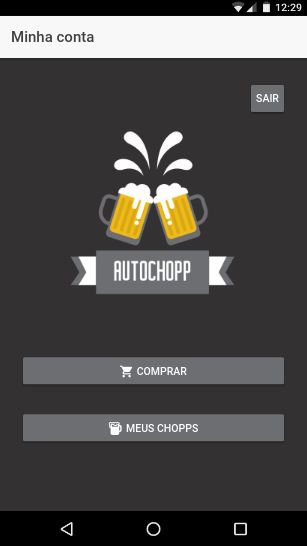
\includegraphics[scale= 0.4]{figuras/home-loged.png}
\caption{Página Inicial - Registrar - Página Inicial com usuário logado. Fonte: Própria.}
\label{telasapp1}
\end{figure}

\begin{figure}[H]
\centering
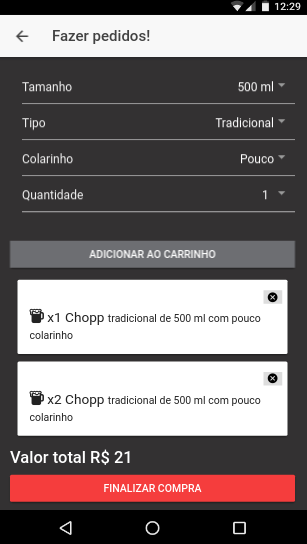
\includegraphics[scale= 0.5]{figuras/pedidos.png}        
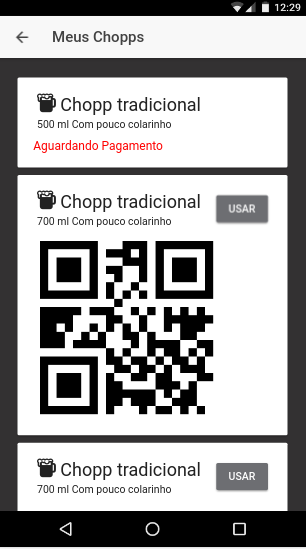
\includegraphics[scale= 0.5]{figuras/MeusChopps.png}
\caption{Tela de Compra - Tela de Pedidos. Fonte: Própria.}
\label{telasapp2}
\end{figure}
